%%%%%%%%%%%%%%%%%%%%%%%%%%%%%%%%%%%%%%%%%
% Programming/Coding Assignment
% LaTeX Template
%
% This template has been downloaded from:
% http://www.latextemplates.com
%
% Original author:
% Ted Pavlic (http://www.tedpavlic.com)
%
% Note:
% The \lipsum[#] commands throughout this template generate dummy text
% to fill the template out. These commands should all be removed when 
% writing assignment content.
%
% This template uses a Perl script as an example snippet of code, most other
% languages are also usable. Configure them in the "CODE INCLUSION 
% CONFIGURATION" section.
%
%%%%%%%%%%%%%%%%%%%%%%%%%%%%%%%%%%%%%%%%%

%----------------------------------------------------------------------------------------
%	PACKAGES AND OTHER DOCUMENT CONFIGURATIONS
%----------------------------------------------------------------------------------------

\documentclass{article}

\usepackage{fancyhdr} % Required for custom headers
\usepackage{lastpage} % Required to determine the last page for the footer
\usepackage{extramarks} % Required for headers and footers
\usepackage[usenames,dvipsnames]{color} % Required for custom colors
\usepackage{graphicx} % Required to insert images
\usepackage{listings} % Required for insertion of code
\usepackage{courier} % Required for the courier font
\usepackage{lipsum} % Used for inserting dummy 'Lorem ipsum' text into the template

\usepackage{float}
\usepackage{amsfonts}
\usepackage{amsmath}
\usepackage{bm}

% Margins
\topmargin=-0.45in
\evensidemargin=0in
\oddsidemargin=0in
\textwidth=6.5in
\textheight=9.0in
\headsep=0.25in

\linespread{1.1} % Line spacing

% Set up the header and footer
\pagestyle{fancy}
\lhead{K. Holmbeck and D. Tonne} % Top left header
\chead{\hmwkClass\ : \hmwkTitle} % Top center head
\rhead{\firstxmark} % Top right header
\lfoot{\lastxmark} % Bottom left footer
\cfoot{} % Bottom center footer
\rfoot{Page\ \thepage\ of\ \pageref{LastPage}} % Bottom right footer
\renewcommand\headrulewidth{0.4pt} % Size of the header rule
\renewcommand\footrulewidth{0.4pt} % Size of the footer rule

\setlength\parindent{0pt} % Removes all indentation from paragraphs

%----------------------------------------------------------------------------------------
%	CODE INCLUSION CONFIGURATION
%----------------------------------------------------------------------------------------

\usepackage{color} %red, green, blue, yellow, cyan, magenta, black, white
\definecolor{mygreen}{RGB}{28,172,0} % color values Red, Green, Blue
\definecolor{mylilas}{RGB}{170,55,241}

\lstset{language=Matlab,%
    basicstyle=\ttfamily\footnotesize,breaklines=true
    %basicstyle=\footnotesize\color{red},
    breaklines=true,%
    xleftmargin=0.5in,
    %xrightmargin=0.25in,
    morekeywords={matlab2tikz},
    keywordstyle=\color{blue},%
    morekeywords=[2]{1}, keywordstyle=[2]{\color{black}},
    identifierstyle=\color{black},%
    stringstyle=\color{mylilas},
    commentstyle=\color{mygreen},%
    showstringspaces=false,%without this there will be a symbol in the places where there is a space
    numbers=left,%
    numberstyle={\tiny \color{black}},% size of the numbers
    numbersep=9pt, % this defines how far the numbers are from the text
    emph=[1]{for,end,break},emphstyle=[1]\color{blue}, %some words to emphasise
    %emph=[2]{word1,word2}, emphstyle=[2]{style},    
}


%----------------------------------------------------------------------------------------
%	DOCUMENT STRUCTURE COMMANDS
%	Skip this unless you know what you're doing
%----------------------------------------------------------------------------------------

% Header and footer for when a page split occurs within a problem environment
\newcommand{\enterProblemHeader}[1]{
%\nobreak\extramarks{#1}{#1 continued on next page\ldots}\nobreak
%\nobreak\extramarks{#1 (continued)}{#1 continued on next page\ldots}\nobreak
}

% Header and footer for when a page split occurs between problem environments
\newcommand{\exitProblemHeader}[1]{
\nobreak\extramarks{#1 (continued)}{#1 continued on next page\ldots}\nobreak
\nobreak\extramarks{#1}{}\nobreak
}

\setcounter{secnumdepth}{0} % Removes default section numbers
\newcounter{homeworkProblemCounter} % Creates a counter to keep track of the number of problems

\newcommand{\homeworkProblemName}{}
\newenvironment{homeworkProblem}[1][Problem \arabic{homeworkProblemCounter}]{ % Makes a new environment called homeworkProblem which takes 1 argument (custom name) but the default is "Problem #"
\stepcounter{homeworkProblemCounter} % Increase counter for number of problems
\renewcommand{\homeworkProblemName}{#1} % Assign \homeworkProblemName the name of the problem
\subsection{\homeworkProblemName} % Make a section in the document with the custom problem count
\enterProblemHeader{\homeworkProblemName} % Header and footer within the environment
}{
\exitProblemHeader{\homeworkProblemName} % Header and footer after the environment
}

\newcommand{\problemAnswer}[1]{ % Defines the problem answer command with the content as the only argument
\noindent\framebox[\columnwidth][c]{\begin{minipage}{0.98\columnwidth}#1\end{minipage}} % Makes the box around the problem answer and puts the content inside
}

\newcommand{\homeworkSectionName}{}
\newenvironment{homeworkSection}[1]{ % New environment for sections within homework problems, takes 1 argument - the name of the section
\renewcommand{\homeworkSectionName}{#1} % Assign \homeworkSectionName to the name of the section from the environment argument
\subsection{\homeworkSectionName} % Make a subsection with the custom name of the subsection
\enterProblemHeader{\homeworkProblemName\ [\homeworkSectionName]} % Header and footer within the environment
}{
\enterProblemHeader{\homeworkProblemName} % Header and footer after the environment
}


%----------------------------------------------------------------------------------------
%   NAME AND CLASS SECTION
%----------------------------------------------------------------------------------------

\newcommand{\hmwkTitle}{Classification: Cats and Dogs} % Assignment title
\newcommand{\hmwkDueDate}{Tuesday,\ May\ 15,\ 2018} % Due date
\newcommand{\hmwkClass}{Math\ 521} % Course/clas
\newcommand{\hmwkAuthorName}{Kristin Holmbeck and Debbie Tonne} % Your name

%----------------------------------------------------------------------------------------
%   TITLE PAGE
%----------------------------------------------------------------------------------------

\title{
\textmd{\textbf{\hmwkClass \ \hmwkTitle}}\\
\normalsize\vspace{0.1in}\small{Due\ on\ \hmwkDueDate}\\
\vspace{0.1in}
\vspace{0.2in}
}

\author{\textbf{\hmwkAuthorName}}
\date{} % Insert date here if you want it to appear below your name

%----------------------------------------------------------------------------------------

\begin{document}

\maketitle

%----------------------------------------------------------------------------------------
%   TABLE OF CONTENTS
%----------------------------------------------------------------------------------------

%\setcounter{tocdepth}{1} % Uncomment this line if you don't want subsections listed in the ToC
\vspace{0.75in}
\tableofcontents
\listoffigures

\newpage

%----------------------------------------------------------------------------------------
%   PROBLEM 1
%----------------------------------------------------------------------------------------

% To have just one problem per page, simply put a \clearpage after each problem

\begin{section}{Theory}

\begin{subsection}{Introduction}
The project we present in this report involves properly classifying two data sets successfully. In this context, the data sets are images of dogs and cats, but the same ideas and algorithms can be successfully applied to other data sets, such as sound waves. Since we are working with images, some preprocessing methods will be explored to add uniformity or variance to the data sets. 
\end{subsection}

\begin{subsection}{Preprocessing}
Image \textit{preprocessing} typically involves filtering or computing the Fourier transform of an image prior to analysis. To this end, we will discuss some basics, beginning with filtering. 
\\
\\
Image filtering uses a \textit{mask} matrix on subsets of an image to perform operations. One filter example is the averaging filter: Given an $m \times n$ mask size, the mask $m_a$will be
$$
	m_a = \frac{1}{mn} \begin{bmatrix} 1 && \cdots && 1 \\ \vdots && \ddots && \vdots \\ 1 && \cdots && 1 \end{bmatrix}
$$
where the filtering operation involves an $m\times n$ neighborhood around each pixel of the original image matrix $A$.

\end{subsection}

\begin{subsection}{Kernel Discriminant Analysis}
Before detailing the kernel classification method, we will provide an intuitive example for explaining why one might want to use KDA over LDA. First, consider the toy problem of two concentric circles of data (Figure \ref{fig:circle_data}).

\begin{minipage}{1.0\textwidth}
    \begin{figure}[H]
    \centering
    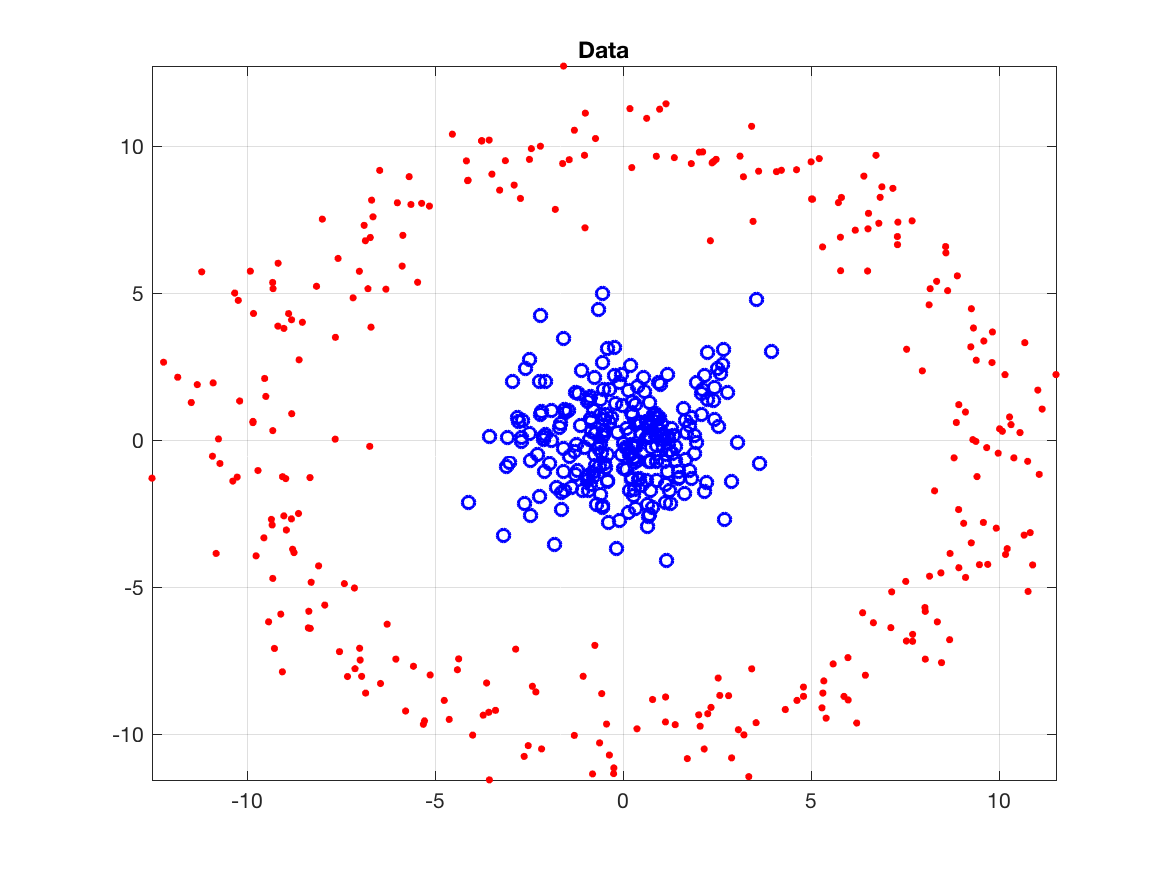
\includegraphics[trim={0cm 0cm 0cm 0cm},clip,width=0.8\columnwidth]{kda_test/circles_data}
    \caption{Concentric Data}
    \label{fig:circle_data}
    \end{figure}
\end{minipage}
\\
\\
\\
There is no way to separate this data linearly, but the classes clearly have a defined separation. Kernel Discriminant Analysis (KDA) utilizes the ideas of LDA but with the data set $X$ mapped onto a new \textit{feature} space $\mathcal{F}$ where the data has a linear relationship in $\mathcal{F}$.
\\
\\
Following the LDA method, suppose our two-class data is given by $X \ X_1 \cup X_2$ where $X_1 = \lbrace x_i \rbrace_{i=1}^{l_1}$ and $X_2 = \lbrace x_j \rbrace_{j=1}^{l_2}$. Now, let $\Phi$ be a nonlinear mapping to some feature space $\mathcal{F}$, that is, we take a vector $x$ from $X$ and map it using $\Phi(x) \in \mathcal{F}$. From the LDA algorithm, we need to maximize
$$
	J(w) = \frac{w^T S_B w}{w^T S_W w}
$$
However, using the new space, we must maximize
$$
	J(w) = \frac{w^T S_B^\Phi w}{w^T S_w^\Phi w}
$$
where 
\begin{align*}
	S_B^\Phi &= (m_1^\Phi - m_2^\Phi) (m_1^\Phi - m_2^\Phi)^T \qquad \text{and} \\
	S_W^\Phi &= \sum_{i=1}^2 \sum_{x \in X_i} (\Phi(x) - m_i^\Phi) (\Phi(x) - m_i^\Phi)^T
\end{align*}
are the between-class and within-class scatter matrices, respectively, in the $\mathcal{F}$ space, and $m_i = \frac{1}{l_i} \sum_{j=1}^{l_i} \Phi( x_j^{(i)} )$, the mean of the $i^{\text{th}}$ class.

\begin{subsubsection}{Kernel Trick}
The kernel trick boils down to using a linear classifier to solve a non-linear problem.
\\
\\
A feature map is a map $\Phi:X \to \mathcal{F}$, where $\mathcal{F}$ is what we call the feature space. Every feature map defines a kernel
$$
	K(x,y) = \langle \Phi(x), \Phi(y) \rangle
$$
where $K$ is clearly symmetric and positive-definite. In the context of linear algebra, the kernel is the space equivalent to the null space. In the statistical context, the kernel is used as a measure of similarity. In particular, the kernel function $k$ defines the distribution of similarities of points around a given point $x$, $k(x,y)$ denotes the similarity of point $x$ with another given point $y$. 
\\

Explicitly computing the mappings of a function $\Phi(x)$ onto $\mathcal{F}$ can become intractable quick. To that end, we instead compute the inner products between the images (images in the linear algebra sense) of all pairs of data in the feature space.
\\
\\
For any $x, \hat{x}$ in $X$, some kernel functions $k(x,\hat{x})$ can be expressed as an inner product in another space $V$. In other words, $k : X \times X \to \mathbb{R}$ and $\Phi : X \to V$.
$$
	k(x, \hat{x}) = \langle \Phi(x), \Phi( \hat{x} ) \rangle_V
$$
\end{subsubsection}

\begin{subsubsection}{KDA on concentric circle data}
Let us revisit the concentric data problem from Figure \ref{fig:circle_data}, and compare the classification of LDA to KDA. For LDA, we obtain the failed classification (Figure \ref{fig:LDA_circles}) and the projection vector along with the data in Figure \ref{fig:LDA_proj_circles}.
\\
\centerline{\begin{minipage}{0.6\textwidth}
    \begin{figure}[H]
    \centering
    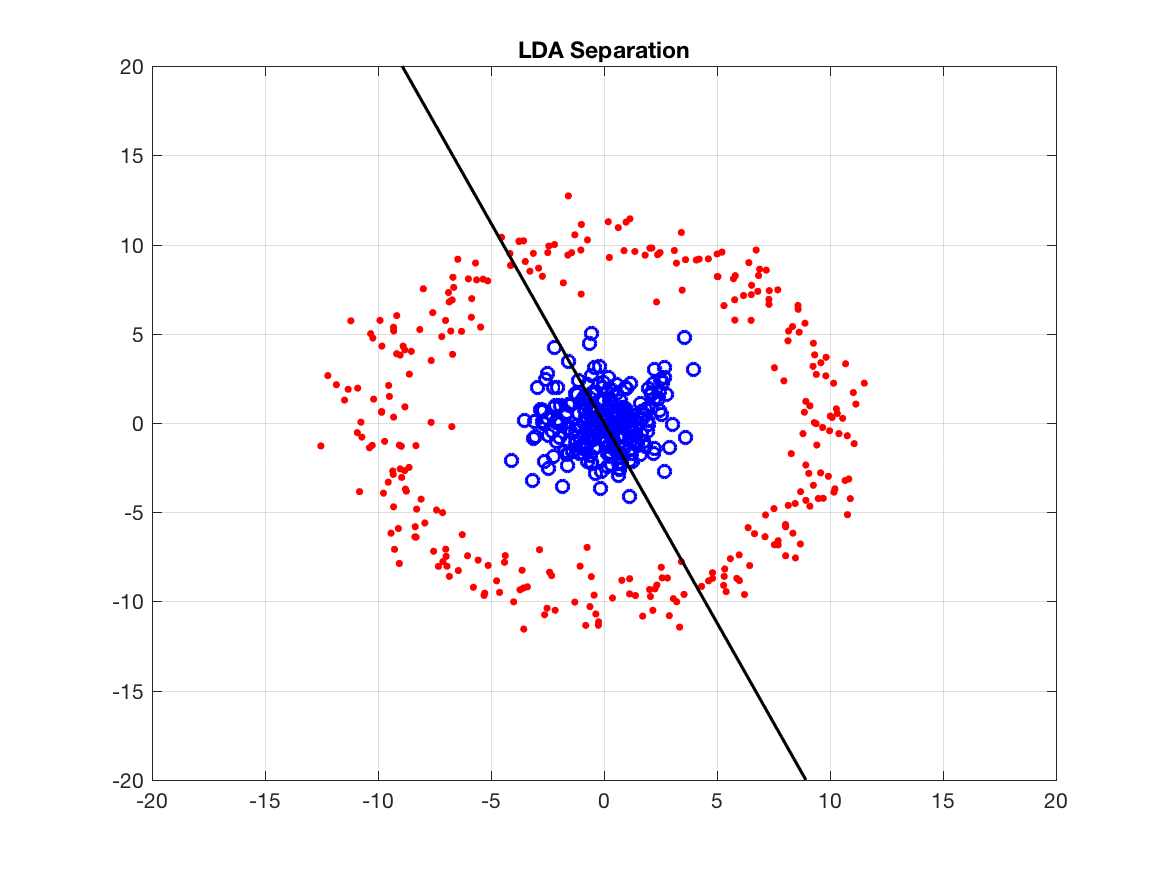
\includegraphics[trim={0cm 0cm 0cm 0cm},clip,width=1.0\columnwidth]{kda_test/LDA_circles}
    \caption{Figure \ref{fig:circle_data} data with LDA projection vector}
    \label{fig:LDA_circles}
    \end{figure}
\end{minipage}}
\centerline{\begin{minipage}{0.6\textwidth}
    \begin{figure}[H]
    \centering
    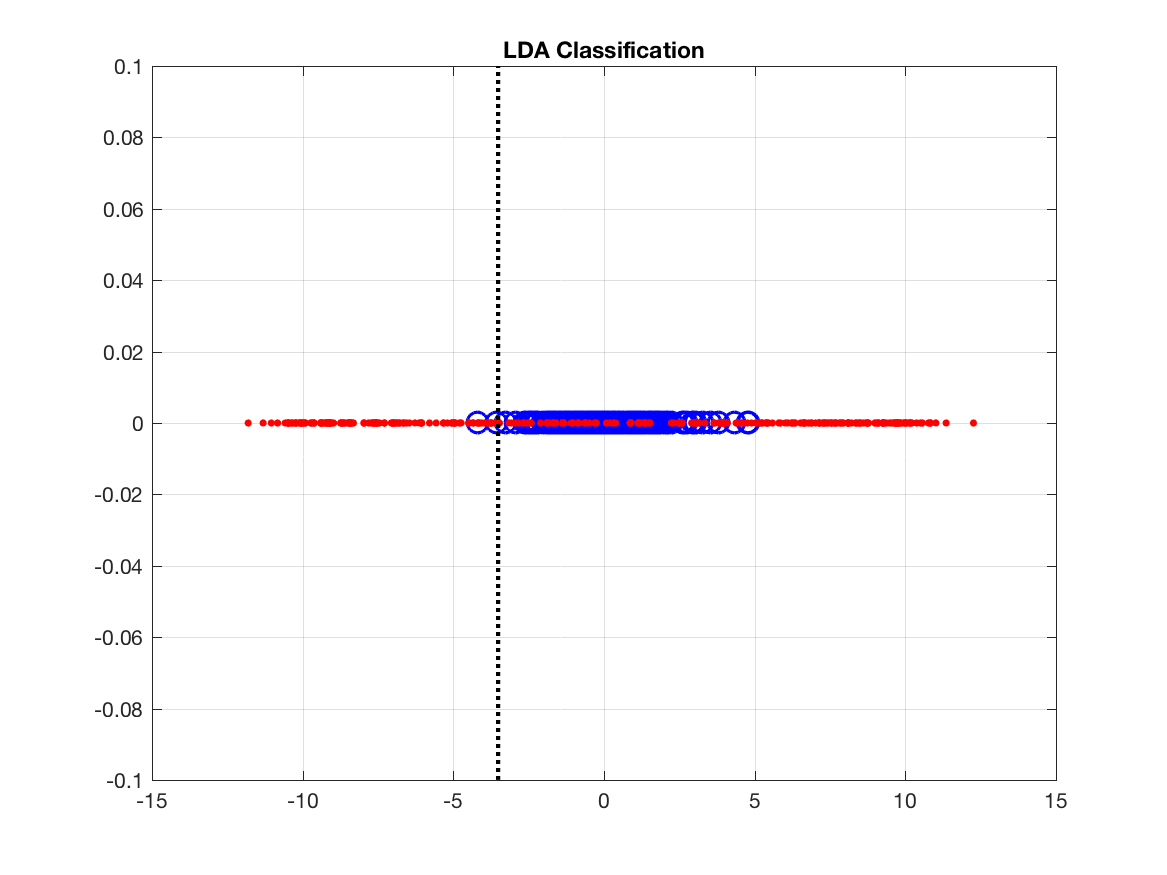
\includegraphics[trim={0cm 0cm 0cm 0cm},clip,width=1.0\columnwidth]{kda_test/LDA_proj_circles}
    \caption{Figure \ref{fig:circle_data} LDA classification}
    \label{fig:LDA_proj_circles}
    \end{figure}
\end{minipage}}
\\
\\
As described above, the kernel conversion is kind of tricky, and thus we cannot plot the equivalent projection vector. However, the successful classification is shown in Figure \ref{fig:KDA_proj_circles}.

\centerline{\begin{minipage}{0.8\textwidth}
    \begin{figure}[H]
    \centering
    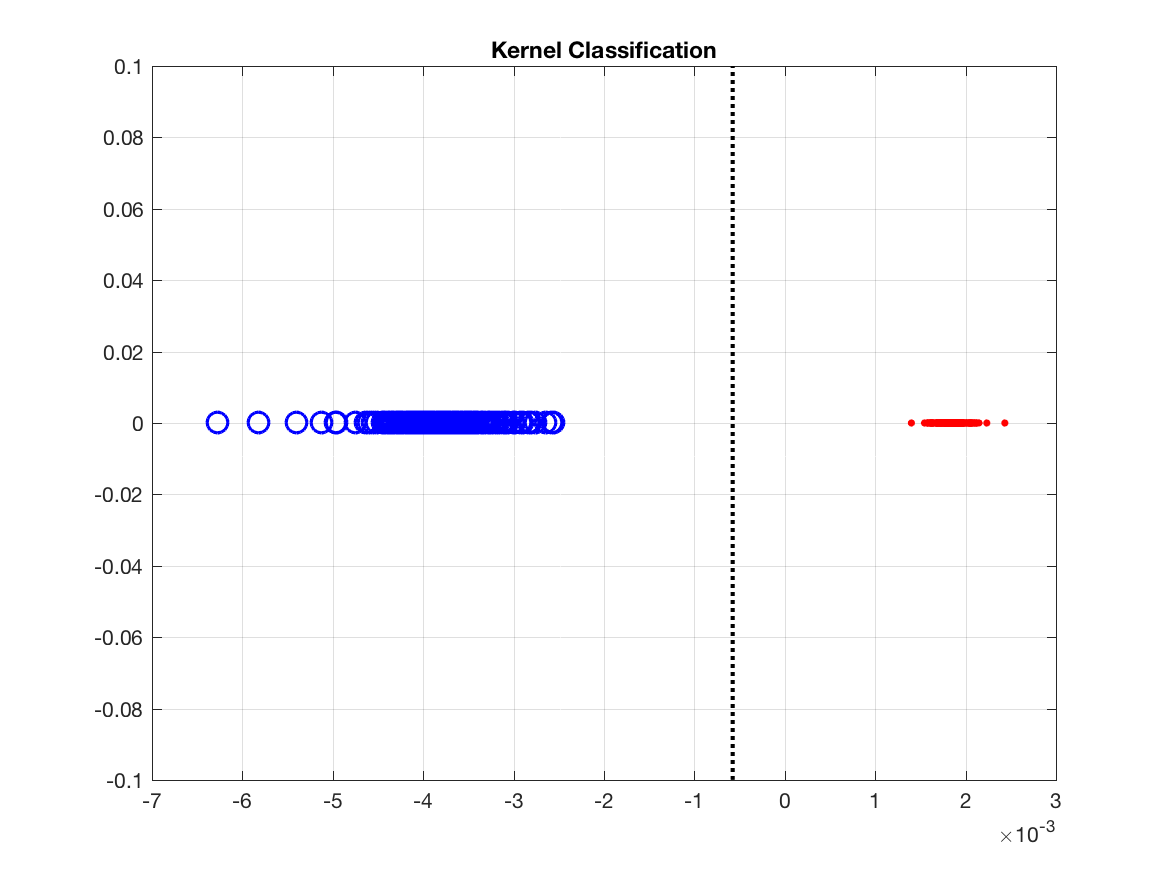
\includegraphics[trim={0cm 0cm 0cm 0cm},clip,width=0.8\columnwidth]{kda_test/KDA_proj_circles}
    \caption{Figure \ref{fig:circle_data} KDA classification}
    \label{fig:KDA_proj_circles}
    \end{figure}
\end{minipage}}

\end{subsubsection}

\begin{subsubsection}{KDA on parabolic data}
Another data set is shown in Figure \ref{fig:parab_data}. Again, this is easily separable, but it's clear that the separation is nonlinear. Again, for LDA, we obtain the failed classification (Figure \ref{fig:LDA_parab}) and the successful classification in Figure \ref{fig:KDA_proj_parab}.
\\
\begin{minipage}{1.0\textwidth}
    \begin{figure}[H]
    \centering
    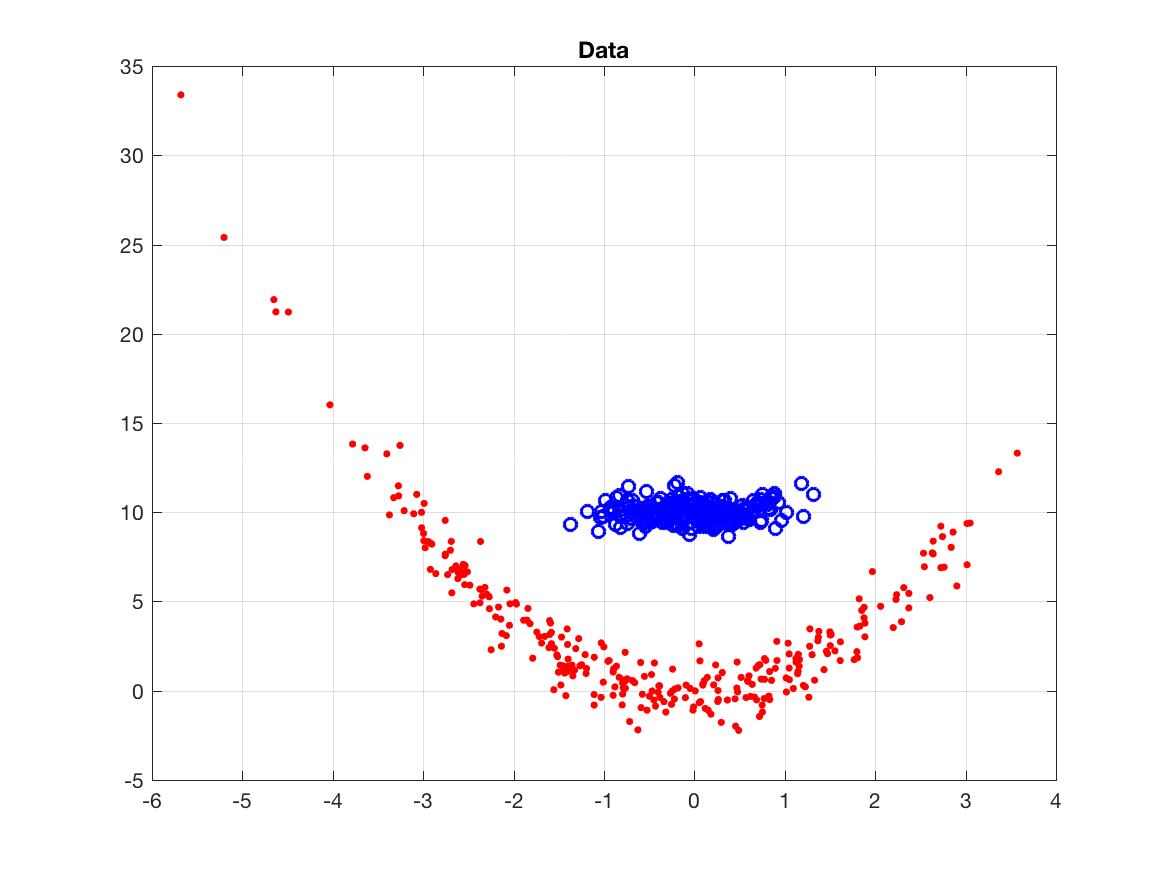
\includegraphics[trim={0cm 0cm 0cm 0cm},clip,width=0.8\columnwidth]{kda_test/parab_data}
    \caption{Parabolically-separable data}
    \label{fig:parab_data}
    \end{figure}
\end{minipage}

\centerline{\begin{minipage}{0.6\textwidth}
    \begin{figure}[H]
    \centering
    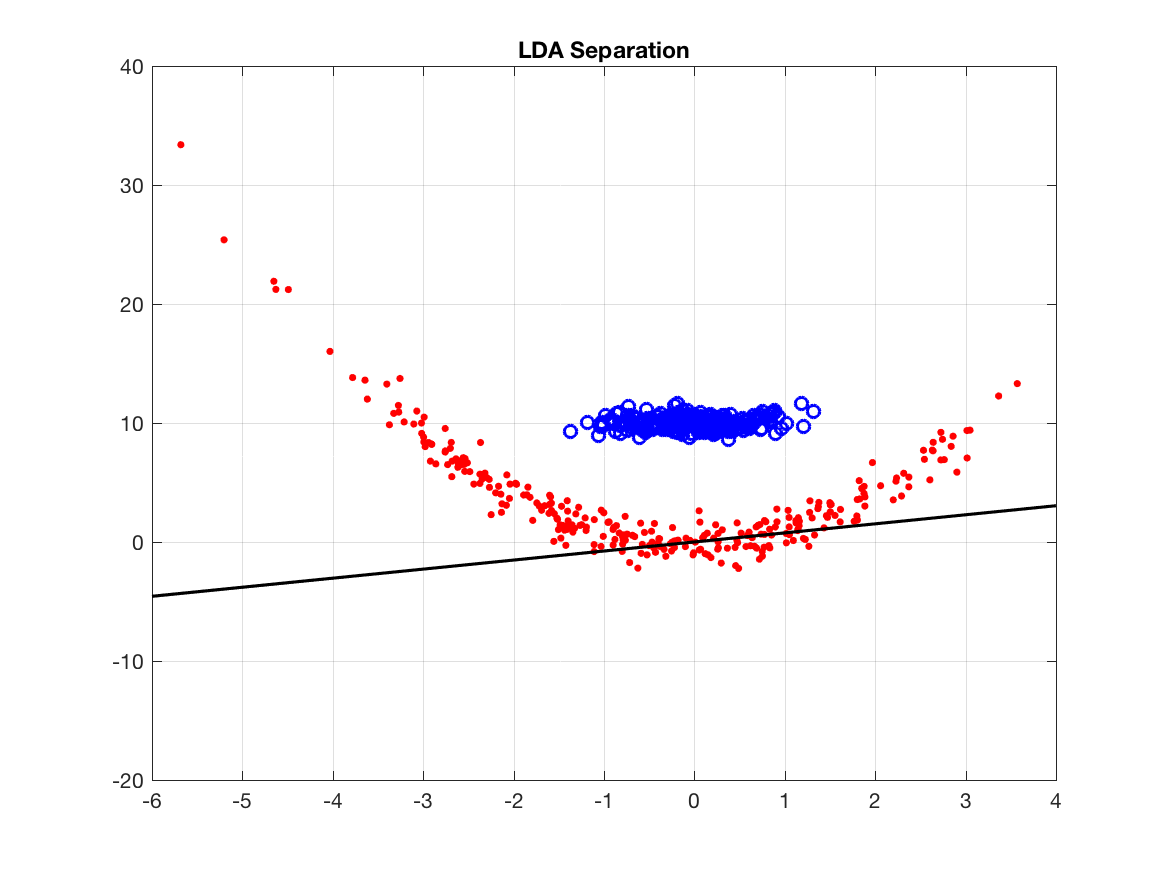
\includegraphics[trim={0cm 0cm 0cm 0cm},clip,width=1.0\columnwidth]{kda_test/LDA_parab}
    \caption{Figure \ref{fig:parab_data} data with LDA projection vector}
    \label{fig:LDA_parab}
    \end{figure}
\end{minipage}}

\centerline{\begin{minipage}{0.6\textwidth}
    \begin{figure}[H]
    \centering
    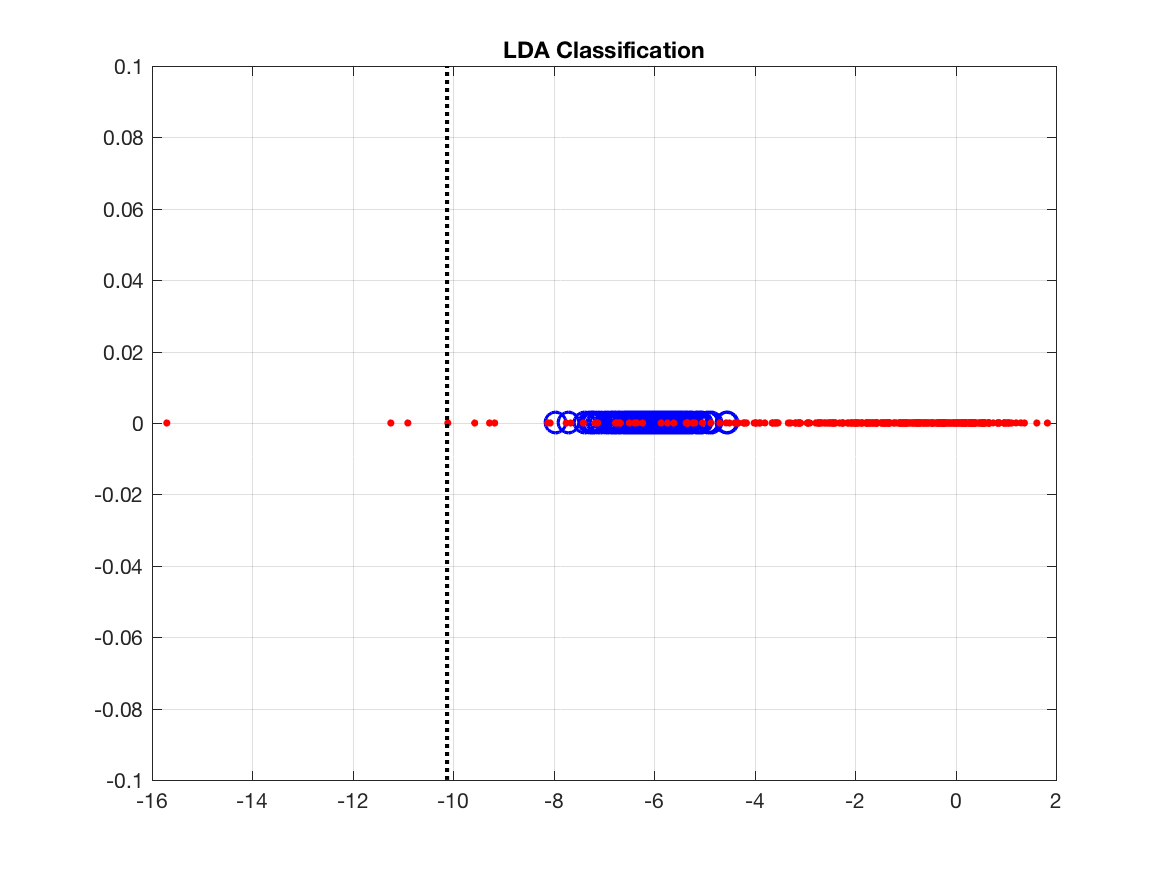
\includegraphics[trim={0cm 0cm 0cm 0cm},clip,width=1.0\columnwidth]{kda_test/LDA_proj_parab}
    \caption{Figure \ref{fig:parab_data} LDA classification}
    \label{fig:LDA_proj_parab}
    \end{figure}
\end{minipage}}

\centerline{\begin{minipage}{0.8\textwidth}
    \begin{figure}[H]
    \centering
    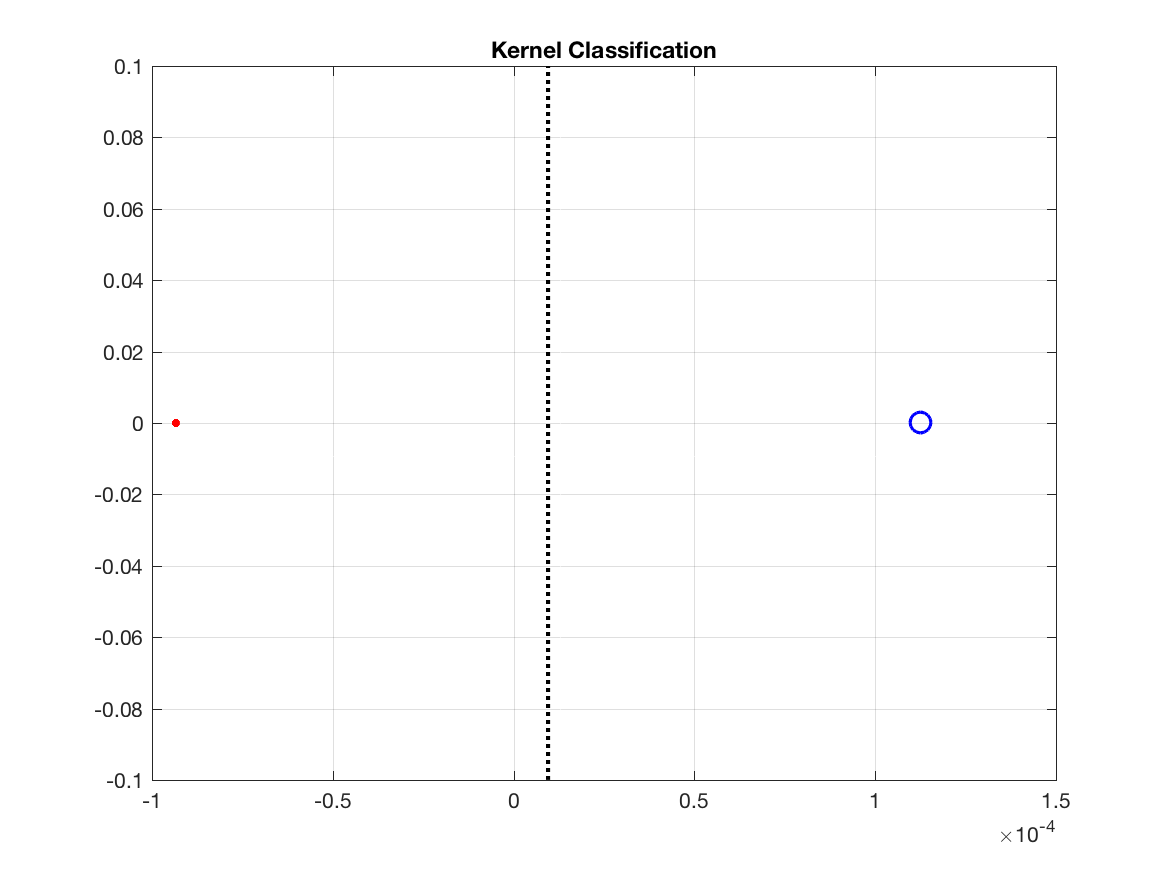
\includegraphics[trim={0cm 0cm 0cm 0cm},clip,width=0.8\columnwidth]{kda_test/KDA_proj_parab}
    \caption{Figure \ref{fig:parab_data} KDA classification}
    \label{fig:KDA_proj_parab}
    \end{figure}
\end{minipage}}
\end{subsubsection}

\end{subsection}



\begin{homeworkSection}{Classification}

\end{homeworkSection}


\begin{homeworkSection}{Singular Values}
The Singular Value Decomposition (SVD) is an important first step in classification.
\end{homeworkSection}

\end{section}


\begin{section}{Results}
\begin{homeworkSection}{Dogs and Cats}
\end{homeworkSection}

\begin{homeworkSection}{Classification Types}

\end{homeworkSection}


\end{section}

%----------------------------------------------------------------------------------------
\newpage

\appendix

\section{Code}\label{code}

%\subsection{Gram-Schmidt} \label{code:gram_schmidt}
%\lstinputlisting{../Kristin_Holmbeck_HW2_GramSchmidt.m}


\begin{thebibliography}{10}
    \bibitem{chang}
    Chang, Jen-Mei. \textit{Matrix Methods for Geometric Data Analysis and Recognition}. 2014.

    \bibitem{kda}
	S. Mika, G. Ratsch, J. Weston, B. Scholkopf, and K. Muller. Fisher discriminant analysis with kernels. In \textit{Proc. IEEE Neural Networks for Signal Processing Workshop}, pages 41–48. IEEE Computer Society Press, 1999.

\end{thebibliography}

\end{document}
